
\section{Results}
\label{sec:result}

\subsection{Statistical Interpretation of the Data}
\label{sec:limits}
The statistical interpretation of data is based on the profiled likelihood ratio test statistic as 
for the SM Higgs boson searches~\cite{lhclimits}. The statistical procedures described in the 
following are implemented in the software packages described in~\cite{roofit,roostat,histfactory} used for this analysis.

\subsubsection{The Likelihood Function}
The compatibility of \textit{background only}  and \textit{signal-plus-background}  hypotheses with the observed data is evaluated.  
%Statistical tests are used to quantify the significance of an observation or to set an exclusion limits, 
%in a search for new phenomena, hypothesis testing is performed by means of two hypothesis: 
%the \textit{background only} $H_0$ and and the \textit{signal-plus-background} $H_1$ hypothesis.  
The \emph{test statistic} defined below is based on a binned likelihood function for the data set $\mathcal{D}$:
\begin{multline}\label{likelihood}
\mathcal{L}(\mathcal{D}\,|\,\mu, \boldsymbol{\theta}) =  \prod_{i} \text{Pois(} n_i\, |\, \mu \cdot s_i(\boldsymbol{\theta}) 
	+ b_i(\boldsymbol{\theta})) \cdot \Gamma(\theta^{stat}_i \,| \,\beta_i) 
	 \cdot \prod_{j}\mathcal{G}(\theta_j^{sys} \, |\, 0, 1) ~ 
\end{multline}
describing how likely is a certain hypothesis given the observation of the data set $\mathcal{D}$.
The signal strength parameter $\mu$ allows for reproducing a continuous set of signal hypotheses with 
different cross-section. The value  $\mu= 0$ corresponds to the background-only hypothesis. 
The vector $\boldsymbol{\theta}$ represents the set of \emph{nuisance} parameters  corresponding to
the statistical ($\theta^{stat}_i$) and systematic ($\theta_j^{sys}$) uncertainties in  the signal and background. 
The functions $s_i(\boldsymbol{\theta})$ and  $b_i(\boldsymbol{\theta})$
represent the expected yield of signal and background  for the bin $i$ of the \mmc distribution histograms.
The function $\mathcal{G}(\theta_j^{sys} ~ | ~ 0, 1)$
is the  Gaussian\footnote{Evaluation of systematic uncertainties is obtained from auxiliary measurements. From Bayes theorem,
	assuming a flat prior and a Gaussian distribution for the measured parameter a Gaussian posterior is obtained.	
}
probability density function (p.d.f.) for the nuisance parameter $\theta_j^{sys}$ with mean~=~0 and $\sigma = 1$.  
The impact of the corresponding systematic uncertainty
on the  signal and backgrounds yields and on the shape of the \mmc invariant mass distributions
 is evaluated separately as described in Section~\ref{sec:Systematics}.
The function  $\Gamma(\theta^{stat}_i | \beta_i)$ is an extended gamma function\footnote{The posterior of a
	Poisson distribution assuming a flat prior is a gamma function}
providing the p.d.f. for the nuisance parameter $\theta^{stat}_i$ associated
to the statistical uncertainty $ \beta_i$ in  bin $i$ of the \mmc distribution.
The values of the nuisance parameter set $\boldsymbol{\theta}$ are associated with  variations of the predicted
signal and background event yields with respect to the nominal prediction.
%are evaluated represent
%the uncertainties on the signal and background yields,  or mass shape of the analysis, those uncertainties 
%are usually measured by auxiliary measure to the analysis, like JES for example, or come from theory uncertainty,
%the single p.d.f. of the parameter $\theta_i$ is assumed Gaussian distributed 
%where and it is only function of the parameter $\mu$ and of the
%nuisance parameter $\boldsymbol{\theta}$. If the hypothesis under test is unlikely to happen with the given dataset the value of 
%$\mathcal{L}$ is decreasing,
%one can define which is the best value of a parameter that describes the data via maximising the likelihood,
%obtaining a so called maximum likelihood estimator. 
The Poisson distributions in equation~\eqref{likelihood} give the probability to observe $n_i$ events in the bin \textit{i} of the \mmc 
distribution histogram:
$$
 \text{Pois(}n_i ~ | ~ \mu \cdot s_i(\boldsymbol{\theta}) + b_i(\boldsymbol{\theta})) =  \frac{(\mu s_i(\boldsymbol{\theta}) 
	+b_i(\boldsymbol{\theta}))^{n_i}}{n_i!} ~ e^{-\mu s_i(\boldsymbol{\theta})  -b_i(\boldsymbol{\theta})} \,.
$$
The \mmc distributions in the b-tagged and b-vetoed categories are analysed separately.
The  implementation of the ABCD method in the likelihood function is based on~\cite{ABCD}
and is described in more detail in Appendix~\ref{appendix:limit}.

\subsubsection{Statistical Combination of Results}
Complementary event categories of a search channel (like the b-tagged and b-vetoed categories) 
can be combined in order to increase the signal sensitivity.
If there are no shared events between the categoriesv the combined likelihood functions is simply the product
of the likelihood of the individual categories. The  convention described in~\cite{lhclimits} is used
to take into account correlations of uncertainties in the two combined categories.
The systematic uncertainties are considered either as fully correlated, which means that the same nuisance parameter
describes the corresponding  systematic effect in both categories,  or as fully uncorrelated, in which case different nuisance parameters are
employed for the two categories. Partially correlated uncertainties are either split into components which are 
(un)correlated or they are defined  to be either fully correlated or uncorrelated, depending on which assumption is the most conservative.



\subsubsection{Exclusion Limit Computation}
To compute the compatibility of the data with a given hypothesis, the \emph{profiled likelihood ratio}~\cite{Asympt} 
\begin{equation}
\tilde{q_{\mu}} ~ = ~ -2 \text{ln} ~ \frac{\mathcal{L}(\mathcal{D}~|~\mu, \hat{\boldsymbol{\theta}}_{\mu})}{\mathcal{L}(\mathcal{D} ~| ~ 
\hat{\mu}, \hat{\boldsymbol{\theta}})}
\quad \text{with the constraint} \quad 0 \leq \hat{\mu} \leq \mu
\end{equation}
is used as test statistic with the likelihood function $\mathcal{L}$ defined in equation~\eqref{likelihood}. $\hat{\mu}$ and $\hat{\boldsymbol{\theta}}$ 
are the global maximum likelihood estimators for $\mu$ and $\boldsymbol{\theta}$ from fit to the dataset $\mathcal{D}$, 
whereas $\hat{\boldsymbol{\theta}}_{\mu}$ is the maximum likelihood estimator of $\boldsymbol{\theta}$ from the fit  with
a fixed signal strength $\mu$. $\tilde{q_{\mu}}$ is increasing with 
increasing disagreement between data and the given $\mu$ hypothesis.
Upper limits on the signal cross-section are then defined as follows:
\begin{enumerate}
%	\item The signal hypothesis with signal strength $\mu$ is assumed, under this assumption a set of MC 
%	\textit{pseudo-data} is generated for different values of $\mu$.
%
%	\item  $\tilde{q_{\mu}}$ is calculated for each of the \textit{pseudo-dataset} and each signal hypothesis generating
%	the expected probability density function for $\tilde{q_{\mu}}$ given $\mu$, 
%	$\text{f}(\tilde{q_{\mu}} ~| ~ \mu, \hat{\boldsymbol{\theta}}_{\mu},H_1)$.
%
%	\item The same procedure is repeated for the null hypothesis: pseudo-data are generated with the distribution 
%	of background only and 	obtain  the $\text{f}(\tilde{q_{\mu}} ~ | ~ \mu = 0, \hat{\boldsymbol{\theta}}_{0}, H_0)$.
%
	\item The probability density functions $P(\tilde{q_{\mu}} \,| \, \text{H}_i)$ of $\tilde{q_{\mu}}$ are determined  under the background-only ($H_0$) and 
	the  signal-plus-background ($H_{\mu}$) hypotheses for  given values of $\mu$.
	Since the determination of these functions by means of Monte Carlo simulation of pseudo-dataset ($\mathcal{D}$)	demands large computing resources,
	the asymptotic approximation formulae described in~\cite{Asympt} are employed.
	

	\item Once the p.d.f. for the background-only and signal-plus-background hypothesis are obtained, 
	it is possible to define for a given dataset $\mathcal{D}$ two probability values (p-values) for  given value of $\mu$.
	These are the probabilities to obtain data less compatible with the considered hypothesis than the 
	actual observation:
	$$
	p_{s+b} = P(\tilde{q_{\mu}} > \tilde{q_{\mu}}^{observed} ~ | ~ H_{\mu})  
	$$
	$$ 
	p_{b} = P(\tilde{q_{\mu}} > \tilde{q_{\mu}}^{observed} ~ | ~ H_0)
	$$
%	The ratio of this two probabilities defines the quantity $CL_{s} = p_{s+b} / p_{b}$ \cite{cls1,cls2}.

	\item If the ratio $CL_{s} = p_{s+b} / p_{b}$~\cite{cls1,cls2} of the two p-values is less than a given value $\alpha$,
	the signal-plus-background hypothesis with the corresponding $\mu$ is said to be excluded at  (1 - $\alpha$) $CL_{s}$ confidence level. 
	The 95\% confidence level upper limit on $\mu$,
	denoted as $\mu^{95}$, is  the smallest value of $\mu$ for which the  $CL_{s} \le 0.05$\,.

\end{enumerate}
%This is a quite complicated prescription, however 
%its interpretation is not so different from the usual Neyman Construction~\cite{} of confidence intervals:
%for each $\mu$ is possible to define $\tilde{q_{\mu}}^{95}$ for which the probability 
%P$(\tilde{q_{\mu}} \geq \tilde{q_{\mu}}^{95} ~ |~ \mu, ~ H_1$) = 5\%, this means that if $H_1$ is true one expects 
%$\tilde{q_{\mu}} \geq \tilde{q_{\mu}}^{95}$ in 5\% of the cases. With this definition $\mu^{95}$ would be the value of $\mu$
%that for the observed data gives $\tilde{q_{\mu}} = \tilde{q_{\mu}}^{95}$, or in other words a p-value of 5\%.
By construction, rejecting all values of $\mu > \mu^{95}$, the signal-plus-background hypothesis will be 
rejected when it is true at most 5\% of the time.
%given the fact that $\tilde{q_{\mu}}$ is increasing with increasing discrepancy of the hypothesis with data.
The $CL_{s}$ limits are considered conservative and  protected against downward  fluctuations of the data.
% For each pseudo-data sample one can calculate then $\mu^{95}$, which is the biggest value of $\mu$ which gives $\tilde{q_{\mu}} > \tilde{q_{\mu}}^{95}$
%
% Generate a large set of pseudo-data under the hypothesis $H_{0}$ and calculate  $\mu^{95}$ for each of them, by construction one would have
%	that if $H_1$ is true for $\mu > \mu^{95}$ one has $\tilde{q_{\mu}} > \tilde{q_{\mu}}^{95}$ only 5\% of the cases.
%	
%So one it is said that the $\mu > \mu^{95}$ are excluded by data under the hypothesis $H_1$ at 95\% of Confidence Level, meaning that 
%for value of $\mu > \mu^{95}$  one would reject the $H_1$ when is true at most 5\% of the time. 
%
The expected median upper-limit and its error are evaluated with the asymptotic approximation formulae under the background-only hypothesis.
The results have been cross-checked using generated pseudo-data instead of the asymptotic approximation formulae for the determination
of the  probability density functions of $\tilde{q_{\mu}}$. 


\subsubsection{Significance Test of the Background Only Hypothesis}
In case an excess of event is observed  in a given mass range with respect to the background model predictions,
the presence of a signal is quantified by the background only p-value,
 i.e. the probability for the background only to fluctuate
and give rise to an excess of event at least as large as the observend one.

To evaluate the significance of an excess the following  test statistic $q_0$ is chosen:
\begin{equation}
q_0 ~ = ~  -2 \text{ln} ~ \frac{\mathcal{L}(\mathcal{D}~|~0, \hat{\boldsymbol{\theta}}_{0})}{\mathcal{L}(\mathcal{D} ~| ~ \hat{\mu}, \hat{\boldsymbol{\theta}})}
 ~ ~ \text{with} ~  \hat{\mu} \ge 0\,.
\end{equation}
The test statistic is defined for a given set of signal hypothesis. To determine the \emph{local} p-value,
the probability density function of $q_0$ is evaluated under the background only hypothesis for a specific signal mass.  
Since the test of the background only hypothesis is made for many different signal masses, the chance to obtain in the full
mass range a p-value smaller than a predetermined value increases, this is called \emph{look elsewhere effect}~\cite{LEE}
and has to be accounted for in local p-value computation. This is done by counting the number of p-value upper fluctuation over
a defined treshold and downgrading the maximum local p-value by this effect, for more detail see~\cite{lhclimits,LEE}.

To convert the p-value into a significance $Z$, the convention of one sided Gaussian tail is adopted:
\begin{equation}
\text{p-value} = \int_Z^\infty \, \frac{1}{\sqrt{2\pi}} e^{-x^2/2} \, dx \,.
\end{equation}
The 5$\sigma$ significance ($Z = 5$) value which  commonly characterize a discovery corresponds to an 
extremely  small $\text{p-value}\,=\, 2.8 \times 10^{-7}\,.$



\subsection{Exclusion Limits on the Signal Production}
The statistical procedure described in section~\ref{sec:limits} is  the general one used for the SM Higgs
boson where only the Higgs boson mass determines the signal properties. For the MSSM further complication
arises:  there are three neutral Higgs bosons contributing to the total signal yield,
in a particular scenario the masses and cross section are defined 
by two parameter $\tan \beta$ and $m_A$. Thus, the previously described procedure
 has to be repeated for each point in the $\tan \beta - m_A$ plane. 
%For a given scenario, 
%a point in the  $\tan \beta - m_A$ plane is excluded with 95\% $CL_{s}$ confidence level if $\mu^{95} \leq 1$ for that point. 
%Only a limited number of $\tan \beta - m_A$ points are generated, 
%a linear interpolation is used to determine the $\tan \beta$ excluded for a given $m_A$.
For the $m_h^{mod}$ scenario exclusion limits at $95\%$ CLs confidence level 
are derived on the cross section for the neutral MSSM Higgs bosons ($A/h/H$) production via gluon fusion and in association
with b-quarks,  the considered Higgs bosons decay is $A$/$H$/$h\to\tau\tau\to \mu e + 4\nu$. 
A scan has been performed over for 15 tan$\beta$ values ranging\footnote{
			The set of  tan$\beta$ values used
			is 5, 8, 10, 13, 16, 20, 23, 26, 30, 35, 40, 45, 50, 55, 60}  
from $\mathrm{tan}\beta=5$ to $\mathrm{tan}\beta=60$.
A point in the  $\tan \beta - m_A$ plane is excluded if $\mu^{95} \leq 1$ for that point.
A linear interpolation is used to determine the excluded $\tan \beta$ for a given $m_A$.
The procedure is repeated for a set of 12 CP-odd Higgs boson masses values $m_A$ ranging from 90 GeV 
to 300 GeV\footnote{ The set of $m_A$ values used is: 90, 100, 110, 120, 125, 130,
			140, 150, 170, 200, 250 and 300 GeV}.
The expected and observed event yields are compared in bins of the \mmc mass distribution. The bin sizes are
 chosen such that the number of events per bin is high enough to justify the use of the 
asymptotic approximation.
Table~\ref{table:final_numbers} compares the expected and the observed event yields in 
 the two event categories at the final
stage of the event selection. Additionally, Figure \ref{fig:mmc_categories} shows the corresponding 
\mmc mass distributions.

\begin{table} [!t]
\centering
%\begin{small}
\renewcommand{\arraystretch}{1.5}
\begin{tabular}{c p{0.5cm} r l l p{1cm} r l l }
\hline
\hline
Sample 	&	& \multicolumn{3}{c}{b-tag category} 		   	 &	& \multicolumn{3}{c}{b-veto category} 		\\
		&	&  N(event)	&	Stat.	&Syst. 	 & 	&  N(event)	&  Stat.& Syst.		\\ 
\hline
\Ztautau        &     	&       418  	&    $\pm$ 6	&$^{+27}_{-27}$  	&       & 54680	& $\pm$ 60  &$^{+3500}_{-3500}$ \\
\ttbar          &       &       330   	&    $\pm$ 10	& $^{+37}_{-35}$ &       & 2159	& $\pm$ 25  &$^{+280}_{-300}$ \\ 
Multijet        &       &       101	&    $\pm$ 15	& $^{+15}_{-15}$  &       & 3930	& $\pm$ 330 &$^{+590}_{-590}$ \\ 
Other	 	&	&	114	&    $\pm $ 9	&$^{+12}_{-12}$  	&	& 4450	& $\pm$ 110 &$^{+250}_{-250}$ \\
Total           &       &       963     &    $\pm$ 21 	&$^{+50}_{-50}$        &       & 65220	& $\pm$ 360 &$^{+3600}_{-3600}$ \\
\hline
Signal  	&	&	144	&    $\pm$ 7	&$^{+24}_{-33}$		&	& 2028  & $\pm$ 27 & $^{+150}_{-100}$	\\
\hline
Data	        &	& -		& - 		& -		& 	&-	&-	&	-	\\
\hline
\hline

\end{tabular}
%\end{small}
\caption{Expected and observed number event yields in the b-tagged and b-vetoed event category after the full event 
selections. The various background and signal expected event yields are normalized
to the integrated luminosity of the data sample (20.3 $fb^{-1}$).
 The notation ``Other'' stands 
for the electroweak processes $\Wlnu$, $\Zll$, diboson and single top quark production.
$\Ztautau$ has been estimated using the embedding technique. 
The uncertainties quoted include the statistical uncertainty (first number) and the systematic uncertainties (second number).
For the prediction of the MSSM Higgs bosons signal yield, $m_A =150$~GeV and $\tan\beta =20$
is assumed in the $m_h^{mod}$ scenario. }
\label{table:final_numbers}
\end{table}

%\begin{table} [t]
%\centering
%\begin{tabular}{c p{0.5cm} r l l p{1cm} r l l }
%\hline
%\hline
%Sample 	&	& \multicolumn{3}{c}{b-tagged category} 		&	& \multicolumn{3}{c}{b-vetoed category} 		\\ 	[0.5ex]
%		&	&  N(event)	&	Stat.	&Syst.  & 	&  N(event)	&  Stat.	& Syst.		\\ [0.5ex]	
%\hline
%\Ztautau        &     	&       418  	&    $\pm$ 6	&	&       & 54680		& $\pm$ 60	&  		\\   [0.5ex]
%\ttbar          &       &       330   	&    $\pm$ 10	&       &       & 2228		& $\pm$ 25	&	  	\\  [0.5ex]
%Multi-jet        &       &       100	&    $\pm$ 15	&       &       & 3940		& $\pm$ 330	&	  	\\  [0.5ex]
%\Wlnu           &       &       10      &    $\pm$ 6    &       &       & 650		& $\pm$ 100	&	  	\\  [0.5ex]
%Dibosons         &       &       13.1    &    $\pm$ 1.8  &       &       & 2921		& $\pm$ 27	&	  	\\  [0.5ex]
%Single Top      &       &       90	&    $\pm$ 6    &       &       & 443		& $\pm$ 15	&	  	\\  [0.5ex]
%\Zll            &       &       0.9     &    $\pm$ 0.8  &       &       & 430		& $\pm$ 40	&	  	\\  [0.5ex]
%Total           &       &       962     &    $\pm$ 16 	&       &       & 65290		& $\pm$ 180	&	  	\\  [0.5ex]
%\hline
%Signal  	&	&		& 		&	&	&		&		&		\\	[0.5ex]
%\hline
%Data	        &	& -		& - 		& -	& 	&	-	&	-	&	-	\\	[0.5ex]
%\hline
%\hline
%
%\end{tabular}
%\caption{Comparison between yield in data and the one expected from the background model, 
%	b-tagged and b-vetoed category are reported separately. }
%\label{table:final_numbers}
%\end{table}

\begin{figure}[tp]
     \begin{center}
%    \subfigure[]{		
            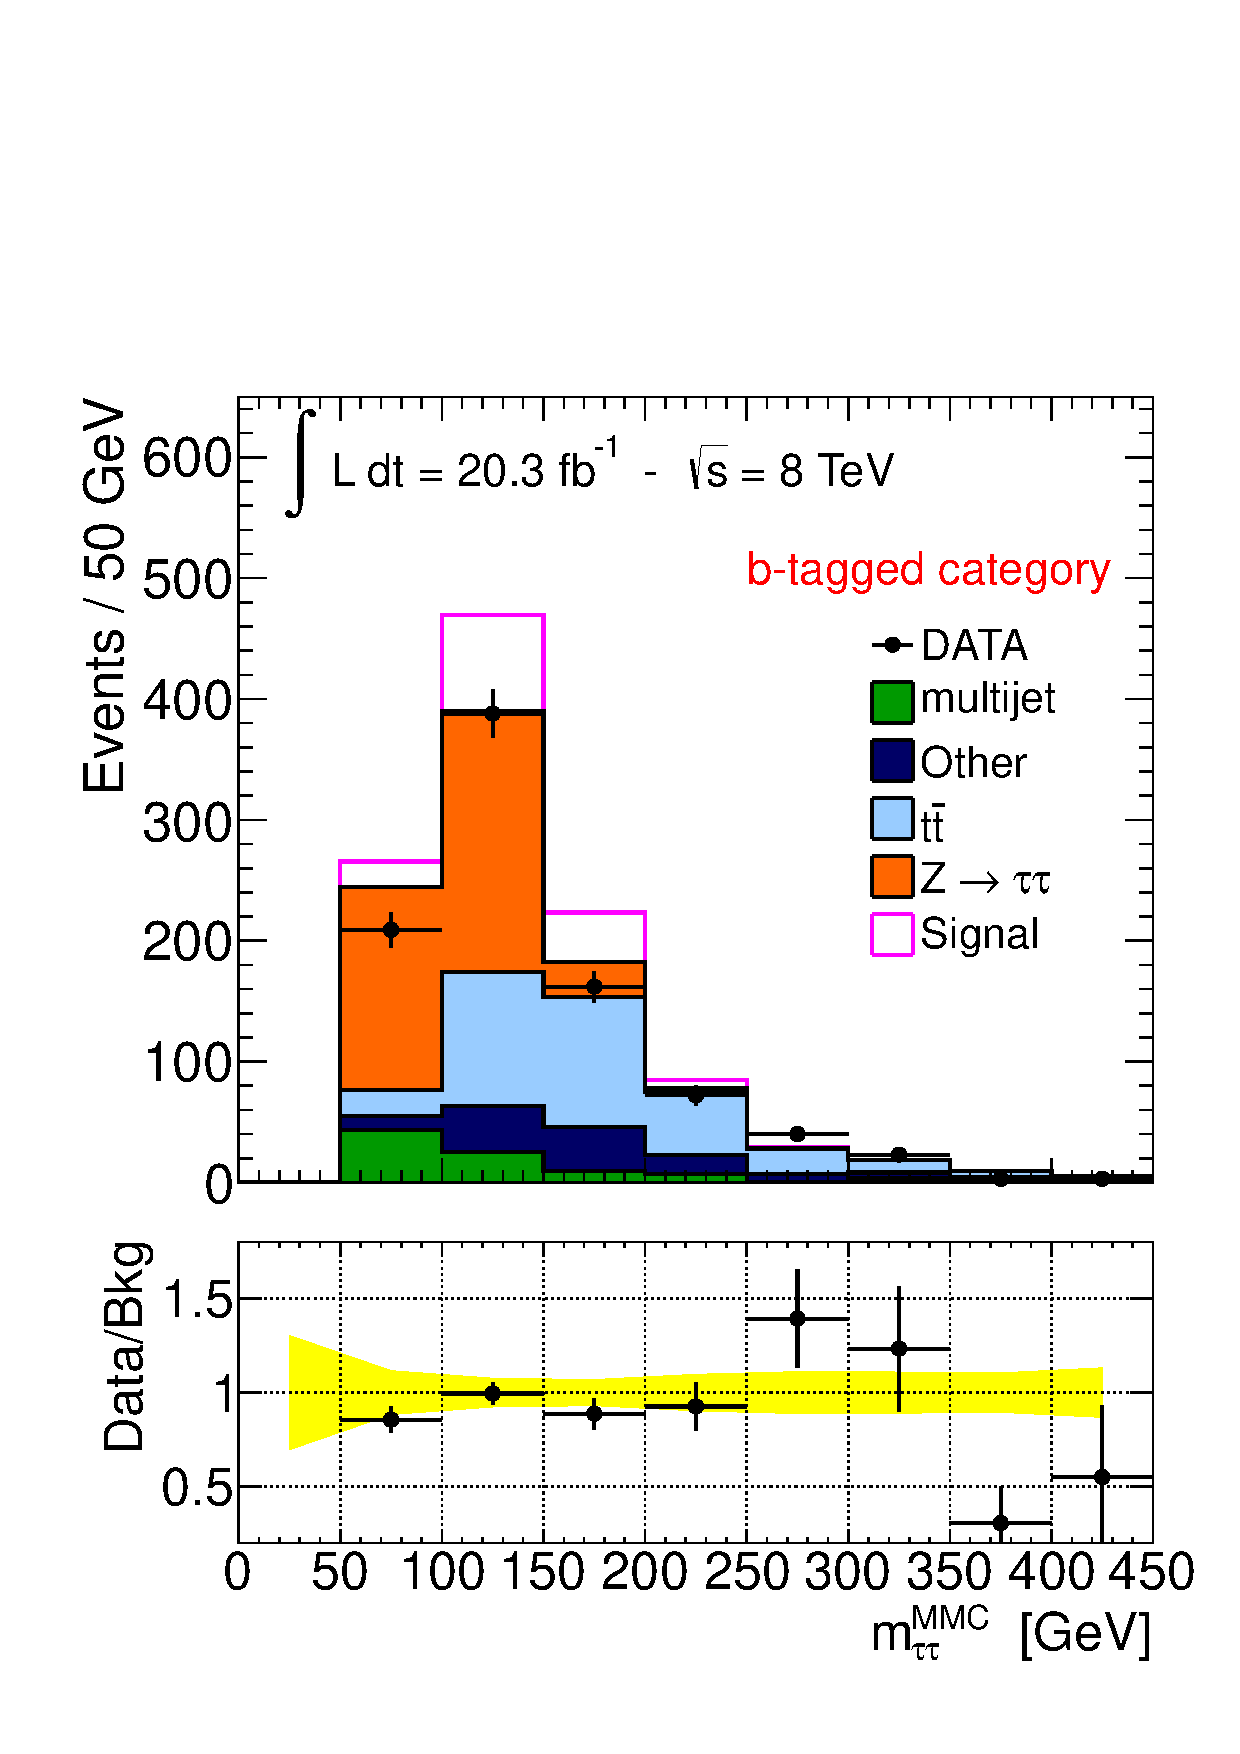
\includegraphics[width=0.47\textwidth]{figure/final_plots/Full_tag_qcd_reg.pdf}
%	    \label{fullbtag2}	
    	%\caption{\footnotesize full b-taggedged.}
 %    }
  %   \subfigure[]{		
            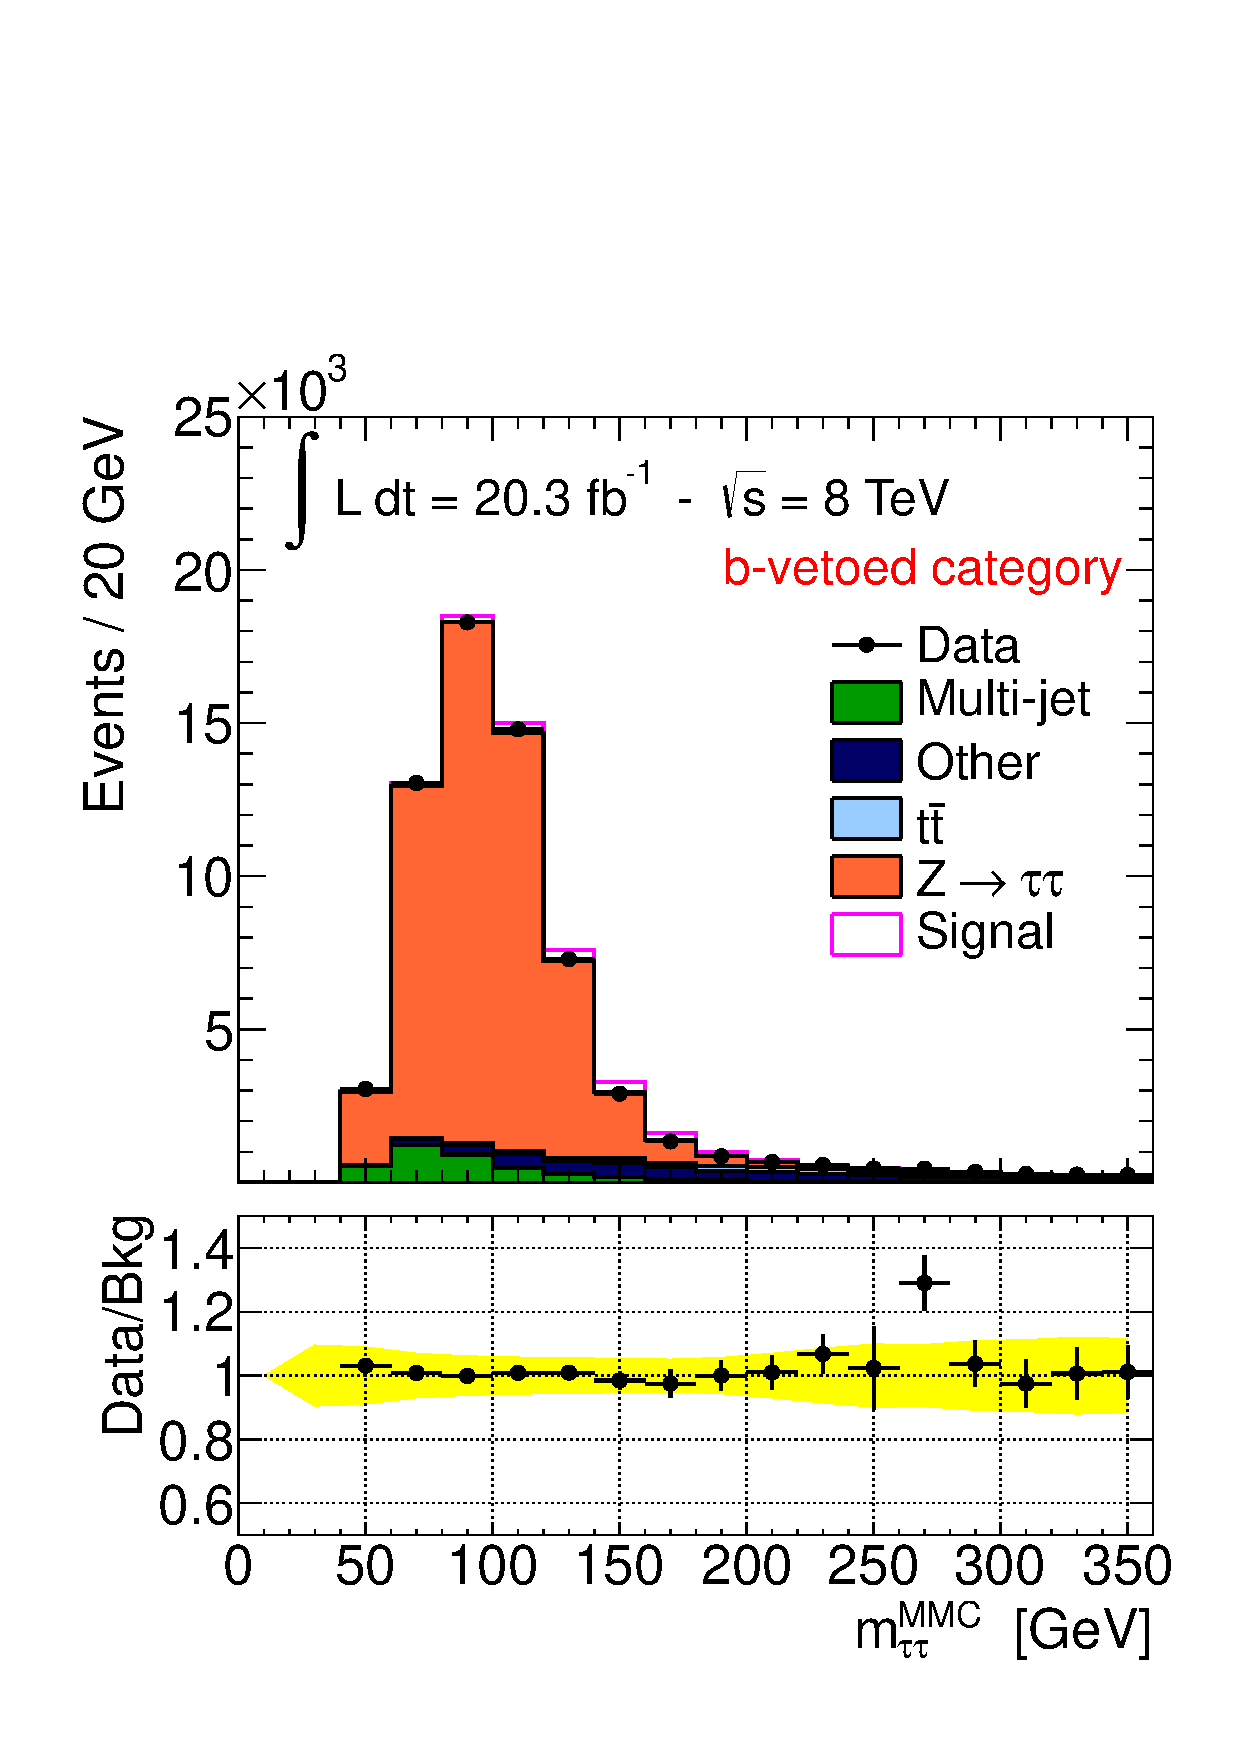
\includegraphics[width=0.47\textwidth]{figure/final_plots/Full_veto_qcd_reg.pdf}
%	    \label{fullveto2}	
    	%\caption{\footnotesize full b-vetoeded.}
   %  }	

    \end{center}
    \caption{ Observed and expected distribution of the \mmc mass for (left) the b-tagged event category and (right) the b-vetoed event category after
        the full event selections. The prediction of the  background model is compared to  data.
	The contribution of the $\Ztautau$ and QCD multi-jet background processes is measured in  dedicated  signal-depleted control data samples,
	the prediction for all the other background processes is obtained from simulation. 
 	 The notation ``Other'' stands 	for the electroweak processes $\Wlnu$, $\Zll$, diboson and single top quark production.
	The prediction for the signal is evaluated considering the production of the three neutral MSSM Higgs bosons in association with b-quarks
	and via the gluon fusion processes in the  $m_{H}^{mod}$ scenario for values of $m_A=150$ GeV and $\tan \beta =20$. 
	The yellow band represents the total systematic uncertainty for the background model prediction.
	}
   \label{fig:mmc_categories}
\end{figure}


The resulting exclusion limit on the MSSM $m_A - \tan\beta$ parameter space are interpreted 
within the $m_{h}^{mod}$ benchmark scenario and  shown in Figure~\ref{fig:limit_extract_combined}. 
The expected and observed exclusion limits at $95\%$ $CL_s$  confidence-level 
are shown as dashed and solid black lines respectively. The green 
and yellow bands correspond to the $1\sigma$ and $2\sigma$ error bands on the expected exclusion limit. 
The analysis is sensitive to the MSSM Higgs boson production for $\tan\beta \geq 13$ and the mass range $90<m_A<200$~GeV.
The observed limit is .... %excludes a CP-odd Higgs with mass $m_A=$140GeV with $\tan\beta \gtrsim$XX.


\begin{figure}[tp]
  \centering
  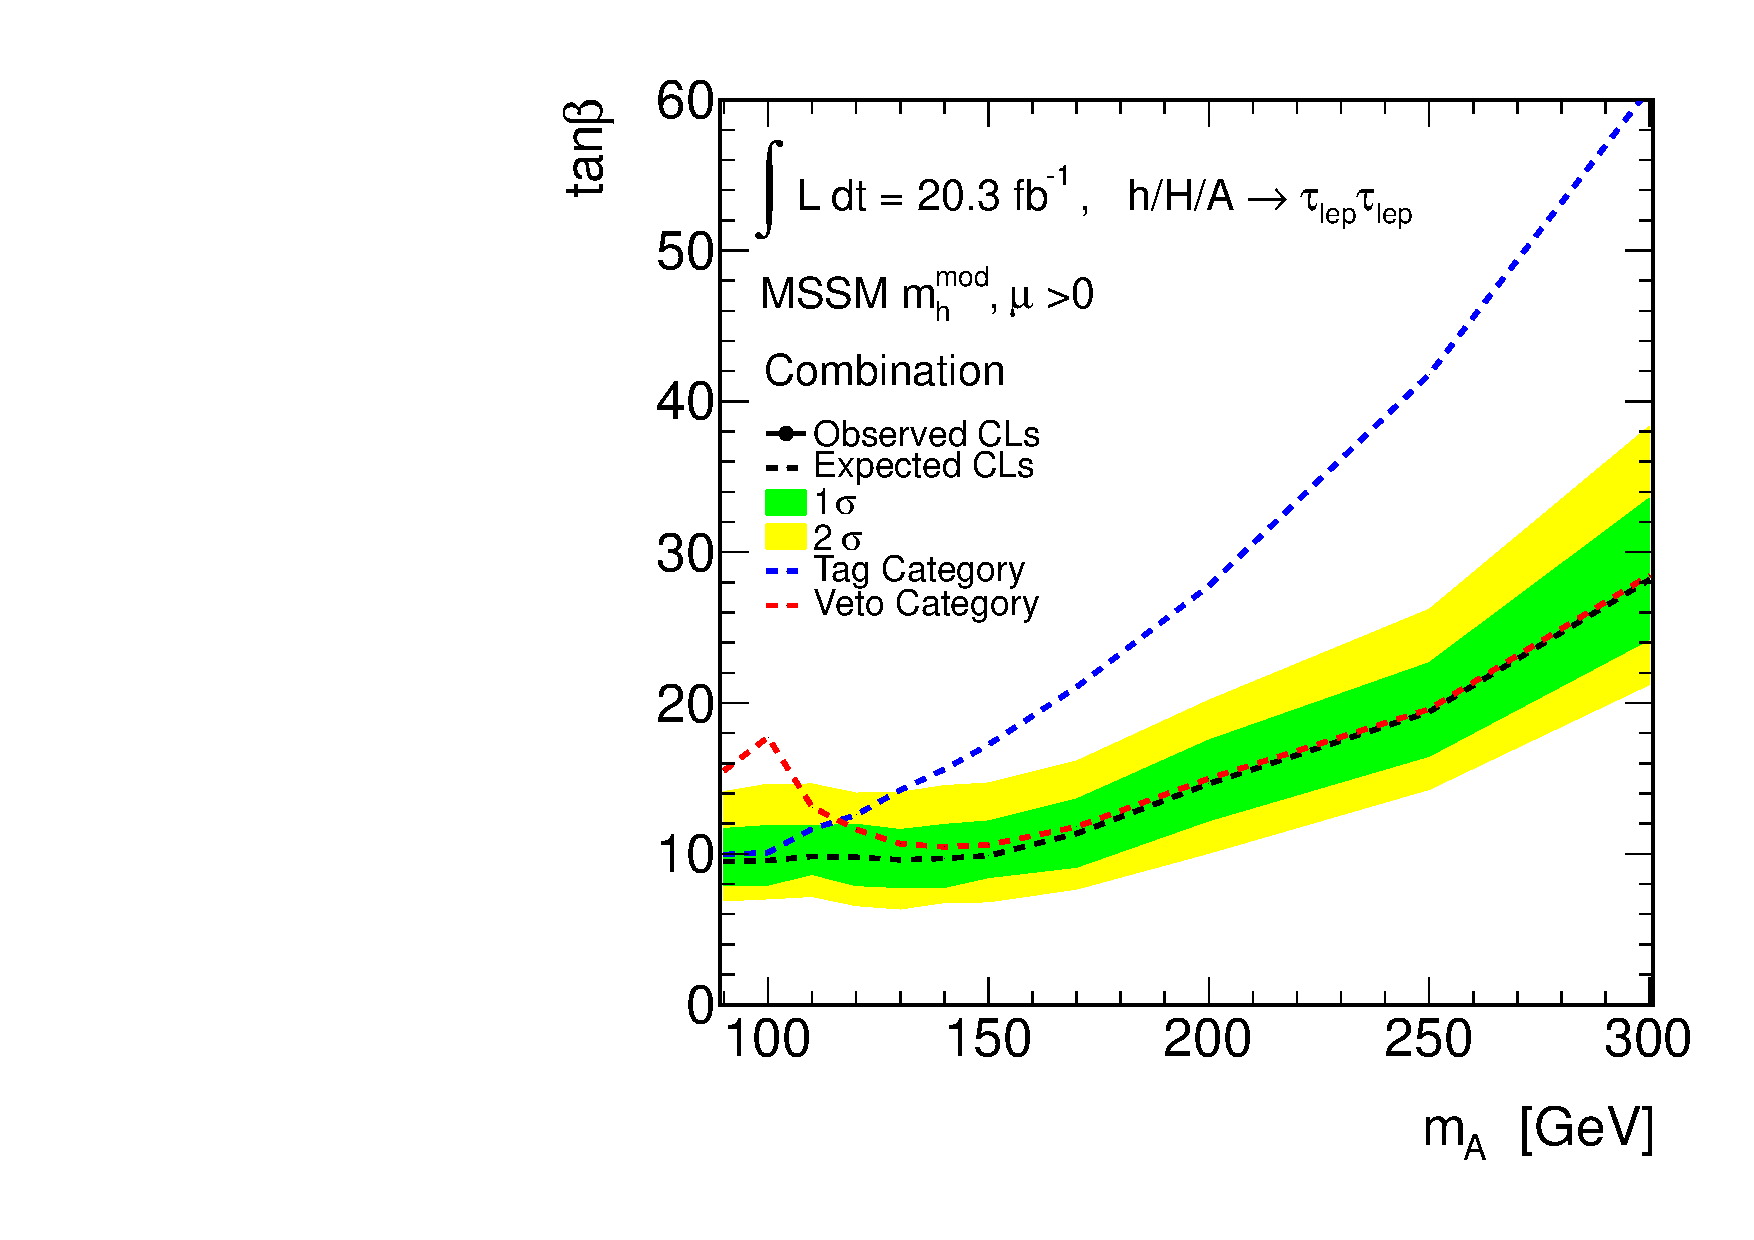
\includegraphics[width=0.8\textwidth]{figure/limits/comb_mit_thesi.pdf}
  \caption{Expected and observed  exclusion limits at the $95\%$ $CL_s$ confidence-level for MSSM Higgs bosons production 
   interpreted in the  $m_A - \tan\beta$ parameter space of the $m_h^{mod}$ scenario. 
	Combined result of the  b-tagged and b-vetoed category is shown.}
\label{fig:limit_extract_combined}
\end{figure}


The outcome of the search is also interpreted in a model-independent way, by setting the limits
on the production cross-section of a scalar boson produced in the
$pp \rightarrow gg \rightarrow \phi$ or $pp \rightarrow bb\phi$ mode and decaying in a di-tau pair.
The corresponding expected and observed $95\%$ $CL_s$ confidence-level  limits are shown in Figure~\ref{fig:limit_xs}.
The limits in the production in association with b-quarks and via gluon fusion are shown separately.
More information on the limit setting procedure and its validation can be found in Appendix~\ref{appendix:limit}.

\begin{figure}[tp]
  \centering
 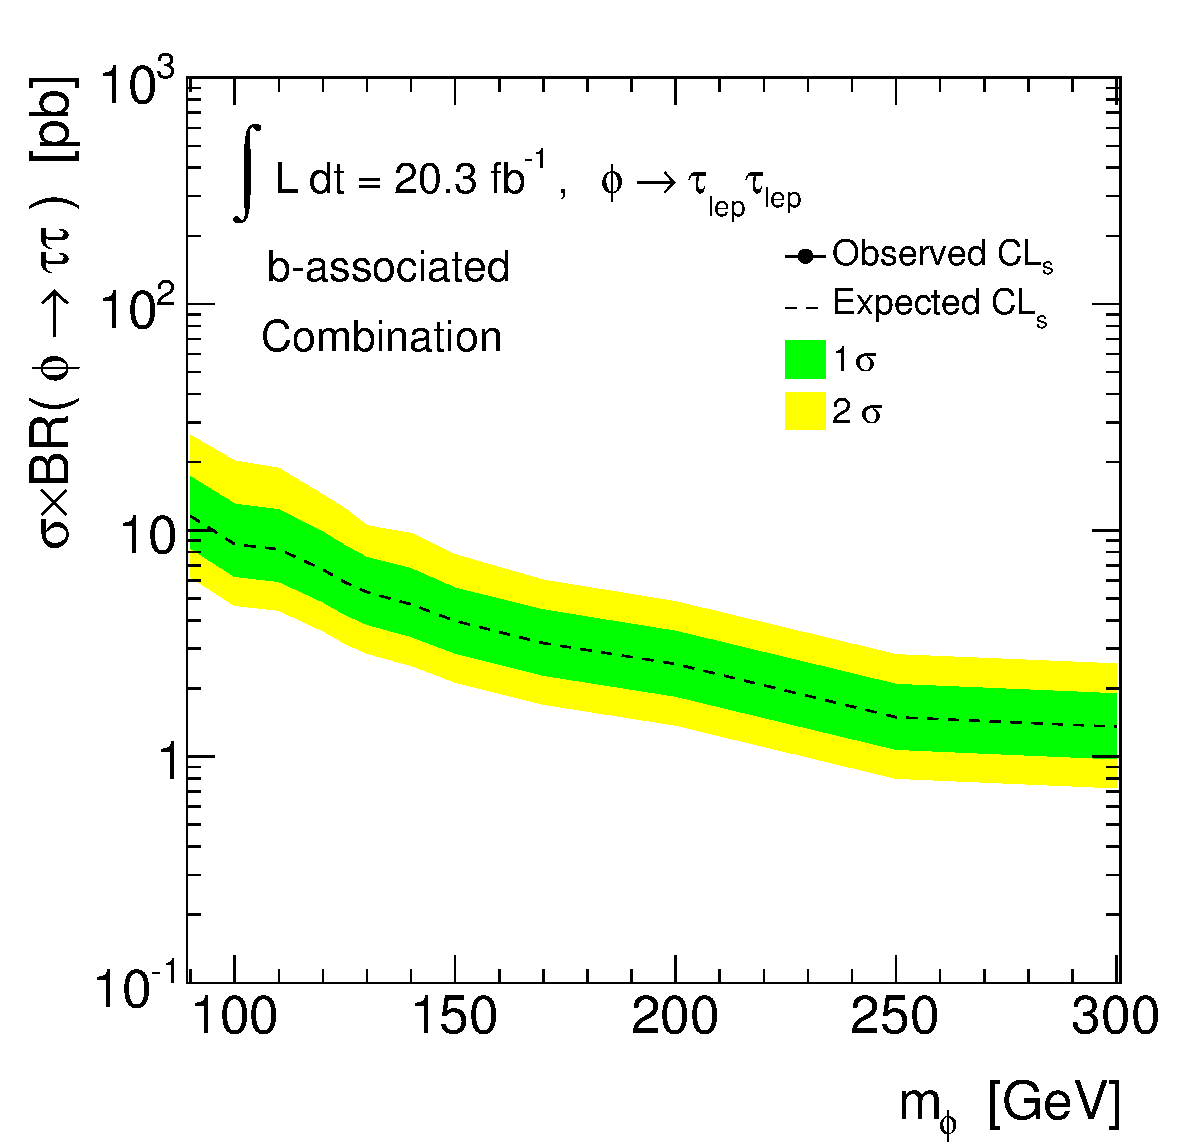
\includegraphics[width=0.6\textwidth]{figure/limits/bbA_combined_thesi.pdf}
 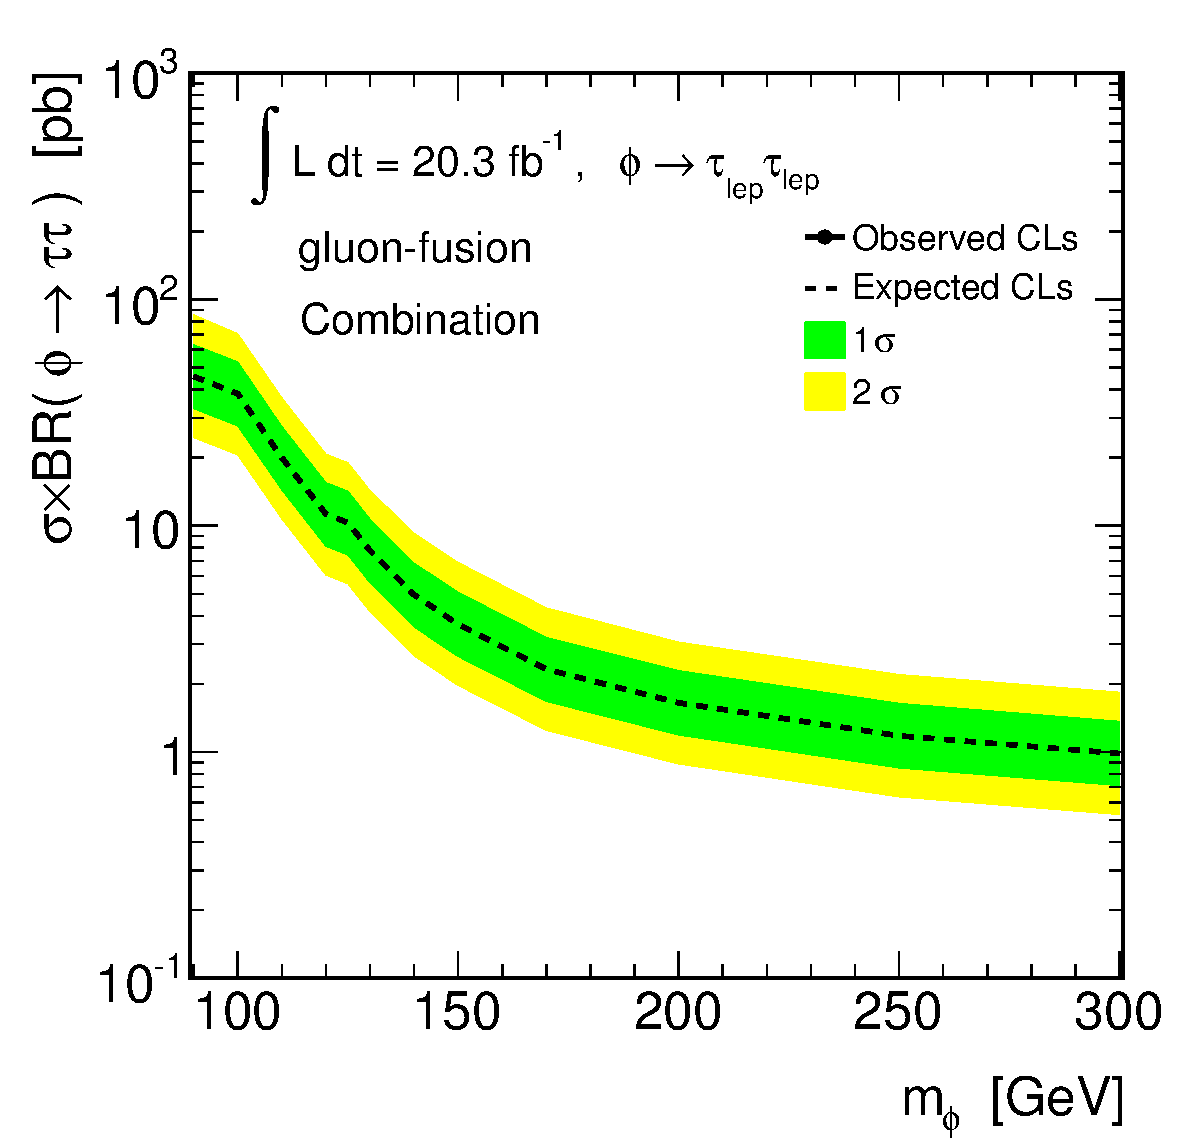
\includegraphics[width=0.6\textwidth]{figure/limits/ggA_comb_thesi.pdf}
  \caption{ Limits on the production of a scalar particle decaying to a di-tau pair
    and produced     in association with b quarks (top) or   via gluon-gluon fusion (bottom).}
\label{fig:limit_xs}
\end{figure}

